\newpage
\chapter{Apache Spark} 

Apache Spark ist ein Open Source Framework, das es ermöglicht verteilt über ein Cluster Programme und Algorithmen auszuführen. Zusätzlich ist das Programmiermodell bzw. die API zum Schreiben solcher Programme sehr einfach und elegant gehalten.\footnote{Vgl. \cite{AAWS15}} \\

\noindent
Das Framework ist im Rahmen eines Forschungsprojekts, welches 2009 in der Universtiy of California in Berkeley im sogenannten AMPLab\footnote{\textbf{AMPLab} ist ein Labor der Berkeley Universität in Californien, die sich auf Big-Data Analysen spezialisiert hat. } ins Leben gerufen wurde, entstanden. Es ist 2010 als Open Source Software unter der BSD-Lizenz\footnote{\textbf{BSD-Lizenz} (Berkeley Software Distribution-Lizenz): bezeichnet eine Gruppe von Lizenzen, die eine breitere Wiederverwertung erlaubt.} zur Verfügung gestellt worden. Das Projekt wird seit 2013 von der Apache Software Foundation\footnote{\textbf{Apache Software Foundation} ist eine ehrenamtlich arbeitende Organisation, die die Apache-Projekte fördert.} weitergeführt. 2014 wurde es als Top Level Projekt eingestuft. Zum aktuellen Zeitpunkt steht Apache Spark unter der Apache 2.0 Lizenz\footnote{Software, die einer \textbf{Apache 2.0 Lizenz} unterliegt, darf bis auf wenige Regeln und Auflagen frei verwendet und verändert werden.} zur Verfügung. \\

%Seit 2010 steht es 

% \ref{sec_sparkr} %\nameref{sec_sparkr} .

\section{Kern-Bibliotheken / Komponenten}

Apache Spark besteht im wesentlichen aus fünf Modulen: Spark Core, Spark SQL, Spark Streaming, Machine Learning Library (MLlib) und GraphX. Zur Nutzung der Komponenten gibt es eine Umfrage aus dem Jahr 2015. Diese ist in \autoref{fig:spark_komp_nutzung} zu sehen. \\

\begin{figure}[h]
  \centering
  \fbox{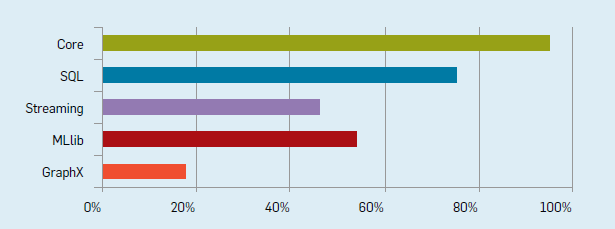
\includegraphics[width=100mm]{./bilder/spark_komponenten_nutzung.png}}	
  \caption{Nutzung der Komponenten \cite{ZXW+16}}\label{fig:spark_komp_nutzung}
\end{figure}


%\newpage
\noindent
Während Spark Core die Kern-Komponente bildet und alle notwendigen Bausteine für das Framework mitbringt, sind die anderen Module auf dem Spark Core Modul aufgebaut und befassen sich mit spezielleren Bereichen wie SQL, Streaming, maschinelles Lernen oder Graphenberechnungen. \autoref{fig:spark_core} zeigt eine Übersicht der Komponenten. \\

\begin{figure}[h]
  \centering
  \fbox{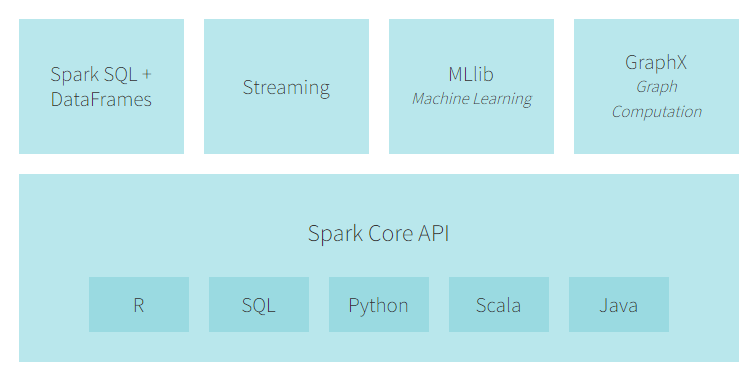
\includegraphics[width=\textwidth]{./bilder/spark_core.png}}
  \caption{Apache Spark Framework \cite{DATABRICK_SPARK_KEY_TERMS}}\label{fig:spark_core}
\end{figure}


\noindent
Die Module werden in den folgenden Kapitel von \ref{sec_sparkcore} bis \ref{sec_sparkmlib} näher betrachtet. \\

\noindent
Darüber hinaus wird in Kapitel \ref{sec_sparkr} SparkR vorgestellt. Das Modul gehört nicht direkt zum Kern, jedoch bietet es die Möglichkeit die Datenanalysen mit R\footnote{\textbf{R} ist eine Programmiersprache für statistische Berechnungen und dem erstellen statistischer Grafiken. } zu optimieren bzw. zu beschleunigen und wird aus diesem Grund mit aufgeführt. \\

\noindent
Den Einsatz der Kern-Komponenten ist im Anhang in \autoref{code:wordcount} zu sehen. In diesem Beispiel werden die 20 meistgenannten Wörter, die in dieser Seminararbeit vorkommen, ermittelt. Dafür wird die Arbeit als PDF eingelesen und in eine Text-Datei konvertiert. Die Zeilen der Datei werden zuerst in Worte aufgeteilt und dann per MapReduce verdichtet und abschließend noch absteigend sortiert.

%Die Aufteilung in die verschiedenen Module macht es sehr gut möglich nur einen Teil der Module zu verwenden. 



\newpage
\subsection{Grundlage des Systems (Spark-Core \& RDD’s)}\label{sec_sparkcore}
%der grundlegende Auführungs-Engine 
Spark Core ist die Grundlage der Spark Plattform. Alle anderen Komponenten bauen auf diesem Kern auf. In dem Kern sind die grundlegenden infrastrukturellen Funktionen enthalten. Darunter zählen die Aufgabenverwaltung, die zeitliche Planung (Scheduling) sowie I/O Funktionen.
Der Kern liefert zum Beispiel die Möglichkeit, Ergebnisse von Berechnungen direkt im Arbeitsspeicher zu halten und diese wiederzuverwenden. Das kann die Geschwindigkeit um das zehn bis 30 fache erhöhen\footnote{Vgl. \cite{VYL+16}}. 
Das grundlegende Programmiermodell besteht aus dem Arbeiten mit den Resilent Distributed Datasets (RDD's). Die API's werden in verschiedenen Sprachen (Java, Scala und Python) bereitgestellt.\footnote{Vgl. \cite{DATABRICK_ABOUT}} In der \autoref{fig:spark_core} sind die einzelnen Bausteine innerhalb der Spark Core Komponenten / API noch einmal im Überblick zu sehen. \\
 

\noindent
Die parallele Verarbeitung wird über den Spark Context realisiert. Der Spark Context wird im Hauptprogramm (Treiberprogramm) erzeugt und ist mit einem Cluster Manager verbunden. Dieser wiederum kennt alle Worker Nodes, welche die Aufgaben ausführen. Die \autoref{fig:spark_cluster} zeigt wie Spark Context, Cluster Manager und die Worker Nodes zusammen agieren. Damit die Aufgaben über viele Nodes verteilt werden können, wird eine Datenstruktur benötigt die dafür ausgelegt ist.\footnote{Vgl. \cite[101]{BDS16}}

\begin{figure}[h]
  \centering
  \fbox{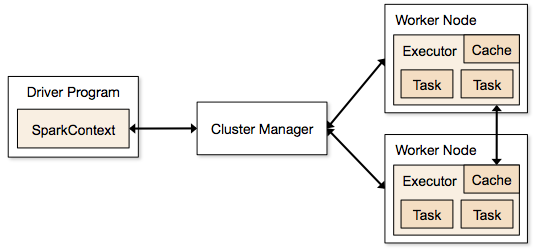
\includegraphics[width=80mm]{./bilder/cluster-overview.png}}
  \caption{Spark Cluster aus \cite{SPCLUSTER}}\label{fig:spark_cluster}
\end{figure}



\noindent
Die RDD's, zu deutsch belastbare, verteilte Datensätze, erledigen diese Aufgabe. Das Dataset ist die primäre Datenabstraktion in Apache Spark. 
Ein RDD entspricht einer partitionierten Sammlung an Daten. Somit können die Partitionen auf verschiedene Systeme (bzw. Worker) verteilt werden.  \\
Nach der Erstellung sind RDD's nur lesbar. Es ist nur möglich ein einmal definiertes RDD durch Anwendung globaler Operationen in ein neues RDD zu überführen. Die Operationen werden anschließend auf allen Partitionen des RDD's auf allen Worker Nodes angewendet. \\
\noindent
Bei den Operationen wird zwischen Transformationen (z.B.: filter oder join) und Aktionen (z.B.: reduce, count, collect oder foreach) unterschieden. Transformationen bilden ein RDD auf ein anderes RDD ab. Aktionen bilden ein RDD auf eine andere Domäne ab.\\ %Todo hier nochmal forschen was das bedeutet
\noindent
Eine Folge von Operationen wird Lineage\footnote{\textbf{RDD Lineage} ist der logische Ablaufplan der einzelnen Operationen. Dadurch können Daten leicht wiederhergestellt werden, falls Fehler aufgetreten sind.} eines RDD's genannt.\footnote{Vgl. \cite{ZC+12}}



\newpage
\subsection{SQL-Abfragen (Spark-SQL \& Data Frames)}\label{sec_sparksql}

%Aus der Spark-Familie ist das die Komponente, die am meisten weiterentwickelt wird. 
Spark-SQL wurde 2014 veröffentlicht. Innerhalb der Spark-Familie wird diese Komponente am stärksten weiterentwickelt. Spark-SQL entstammt dem Apache-Shark. Dadurch sollten folgenden Probleme, die es in Apache Shark gab, gelöst bzw. verbessert werden.
\begin{enumerate}
	\item Mit Apache Shark ist es nur möglich auf Daten im Hive\footnote{\textbf{Apache Hive} ist eine Erweiterung für Hadoop und ermöglicht Abfragen über SQL zu nutzen.} Katalog zuzugreifen. 
	\item Shark lässt sich nur über selbst geschriebene SQL Abfragen aufrufen. 
	\item Hive ist nur für MapReduce optimiert
\end{enumerate}

\noindent
Es werden zwei wesentliche Anwendungsfälle kombiniert. Zum einen ermöglicht es relationale Datenbank-Anfragen zu schreiben und zum anderen prozedurale Algorithmen einzusetzen. 
Dafür werden neben den RDD's die DataFrames als weitere Datenstruktur eingeführt.\\

\noindent
Die Abfragen werden zuerst in den DataFrame-Objekten gespeichert. Erst nach der Initialisierung werden diese SQL Abfragen dann ausgewertet. Für die Auswertung und Optimierung kommt Catalyst\footnote{\textbf{Catalyst} ist eine Optimierungsengine für relationale Ausdrücke.} zum Einsatz. Nach der Auswertung werden die Abfragen gegebenenfalls optimiert und danach in RDD's überführt. In \autoref{fig:spark_sql} sind die Phasen vom SQL-Query bis hin zu den RDD's dargestellt. In den Boxen mit abgerundenten Ecken befinden sich Catalyst-Trees.

\begin{figure}[h]
  \centering
  \fbox{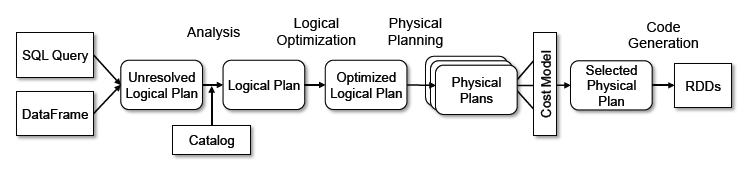
\includegraphics[width=\textwidth]{./bilder/spark_sql.png}}
  \caption{Phasen der Query Planung in Spark SQL \cite{AXL+15}}\label{fig:spark_sql}
\end{figure}

\noindent
Mit Spark-SQL kann ein Zugriff auf relationale Datenbanken erfolgen. Es wurde eine hohe Performance aufgrund etablierter DBMS-Techniken erreicht.
Neue Datenquellen lassen sich leicht anschließen und integrieren.
Zusätzliche Erweiterungen wie maschinelles Lernen und Berechnungen von Graphen sind nutzbar.\footnote{Vgl. \cite{AXL+15}} \\







\newpage
\subsection{Verarbeitung von Datenströmen (Spark-Streaming)}

%Hier nochmal nachlesen, das sieht ganz gut aus. https://www.infoq.com/articles/apache-spark-streaming

Die Spark-Streaming Bibliothek ermöglicht das Verarbeiten von Datenströmen. Dabei dienen RDD's als Grundlage. Die RDD's werden zu DStreams erweitert. DStreams (discretized streams) sind Objekte, die Informationen enthalten, die in Verbindung mit der Zeit stehen. DStreams verwalten intern eine Sequenz von RDD's und werden aus diesem Grund diskrete Streams genannt.
Auch DStreams haben die bereits aus \ref{sec_sparkcore} bekannten zwei Operationen (Transformation und Aktion). \\

\noindent
Um Datenströme zu empfangen wird ein Empfänger (Receiver) auf einem Worker-Knoten gestartet. Die eingehenden Daten werden in kleinen Datenblöcken gespeichert. Dafür werden die Daten innerhalb eines vorgegebenen Zeitfensters gepuffert. Pro Zeitfenster werden die Daten in dem Puffer in eine Partition eines RDD abgelegt.\footnote{Vgl. \cite{BDS16}} \\

\noindent
In der Spark-Streaming Bilbliothek sind bereits einige Empfänger wie Kafka\footnote{\textbf{Apache Kafka} dient zur Verarbeitung von Datenströmen.} und Twitter enthalten. \\
\autoref{fig:spark_streaming} zeigt den Ablauf vom Eingang der Daten über die Verarbeitung bis hin zur Ausgabe. Diese Daten können zum Beispiel auf einem Dashboard ausgegeben oder in einer Datenbank gespeichert werden.

\begin{figure}[h]
  \centering
  \fbox{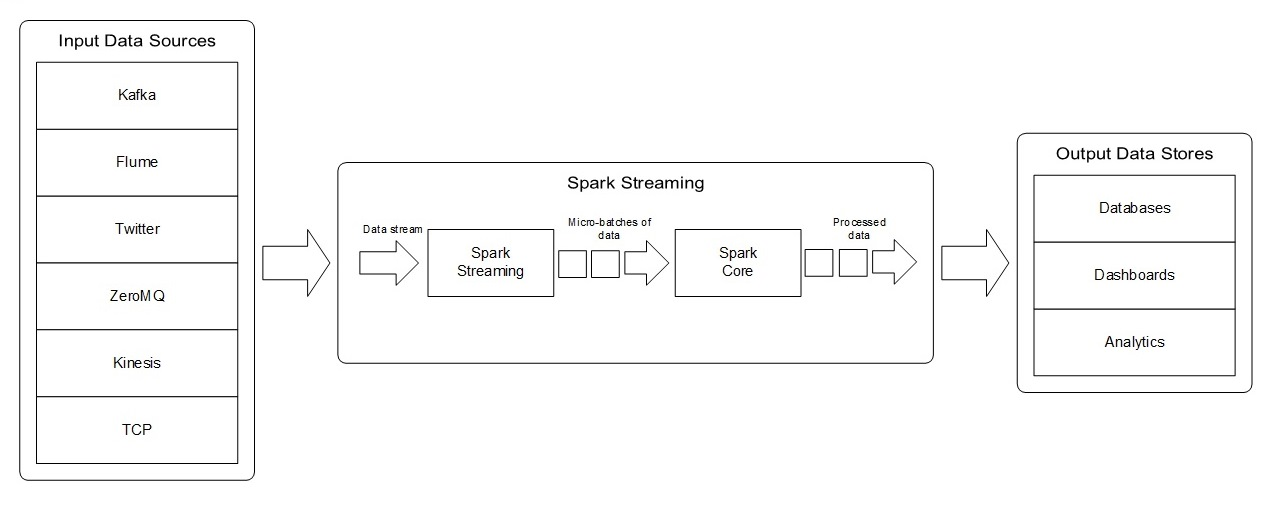
\includegraphics[width=\textwidth]{./bilder/spark_streaming.jpg}}
  \caption{Spark Streaming Ablauf \cite{INFOQ_STREAMING}}\label{fig:spark_streaming}
\end{figure}





\newpage
\subsection{Berechnungen auf Graphen (GraphX)}

Das GraphX Framework ermöglicht die Berechnungen auf Graphen. Die Grundlage sind die RDD's. Als Graphenstrukturen werden Property-Graphen genutzt.
Das sind gerichtete Multigraphen. Das bedeutet, der Graph besteht aus Ecken (Knoten, Vertex) und Kanten (Edge). An den Kanten können Eigenschaften hinterlegt sein.\\

\noindent
In dem GraphX Framework werden diese Graphen aus RDD-Tupeln gebildet. In dem ersten RDD sind die Ecken und in dem zweiten die Kanten enthalten. Um die Graphen auf mehrere Maschinen zu verteilen, werden diese entlang der Kante geteilt. Es handelt sich um das sogenannte Edge Cut Verfahren. Eine einzelne Ecke kann somit auf mehreren Maschinen existieren. Um Änderungen an einer Ecke über alle Kopien auf den Maschinen zu propagieren, wird zusätzlich eine Routing-Tabelle gepflegt. Über diese sind alle Kopien von Ecken bekannt und bei Änderungen einer Ecke werden alle Maschinen entsprechend informiert. 
In der folgenden \autoref{fig:spark_graphx} ist ein verteilter Property-Graph sowie die dazugehörigen Tabellen dargestellt. Zusätzlich sind die verschiedenen RDD's für Knoten(Vertex), Kanten(Edge) und die Routing-Tabelle abgebildet.\footnote{Vgl. \cite{AAWS15}} \\

\begin{figure}[h]
  \centering
  \fbox{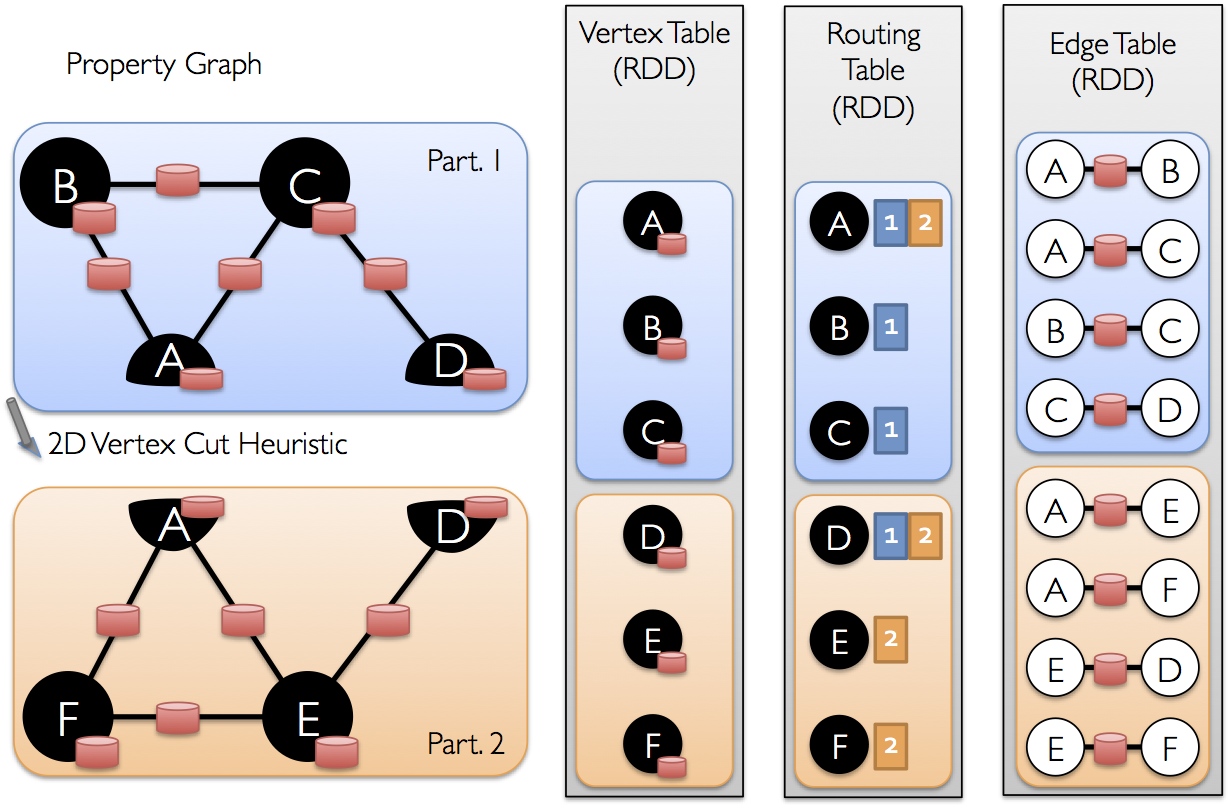
\includegraphics[width=100mm]{./bilder/vertex_routing_edge_tables.png}}
  \caption{Property-Graph mit den dazugehörigen RDD's \cite{SPGRAPHX}}\label{fig:spark_graphx}
\end{figure}

\noindent
Mit Hilfe dieser Technik ist es möglich große Graphen zu zerteilen und auf die Maschinen zu verteilen um dort die gewünschten Operationen durchzuführen. Über die verschiedenen Tabellen können nach der Bearbeitung der Aufgaben die Teil-Graphen wieder zusammengeführt werden. Auch Ausfälle einzelner Nodes oder Datenverluste können somit korrigiert werden. \\



\newpage
\subsection{Maschinelles Lernen (MLlib)}\label{sec_sparkmlib}

MLlib(Machine Learning library) ist eine Bibliothek für maschinelles Lernen. Diese bietet die Möglichkeit, typische maschinelle Lern-Algorithmen auf verteilten Spark-Systemen zu nutzen. Zur Datenabstraktion wird das bereits in \ref{sec_sparksql} erwähnte DataFrame genutzt.  \\

\noindent
In einem Maschinenlernprogramm läuft eine Sequenz von Algorithmen, einer sogenannten Pipeline, ab um die Daten zu verarbeiten und davon zu lernen. 
Dafür gibt es in der MLlib Transformers und Estimator als Pipeline-Komponenten.
Die Transformers verändern die DataFrames. Das Dataframe wird gelesen, die Daten werden anders strukturiert oder aufbereitet und in einem neuen DataFrame wieder ausgegeben. Diese nutzen die Methode \textsl{transform()}.\\
Die Estimators sind Abstraktionen eines Lernalgorithmus. Sie erzeugen Transformer aus dem übergebenen DataFrame. Diese Estimator nutzen die Methode \textsl{fit()}.
Eine Pipeline selbst ist wiederum ein Estimator.\footnote{Vgl. \cite{AAWS15}} \\

\noindent
Das Zusammenspiel zwischen Trasformers und Estimators ist in der \autoref{fig:spark_ml_pipeline} beispielhaft dargestellt. \\
 
\begin{figure}[h]
  \centering
  \fbox{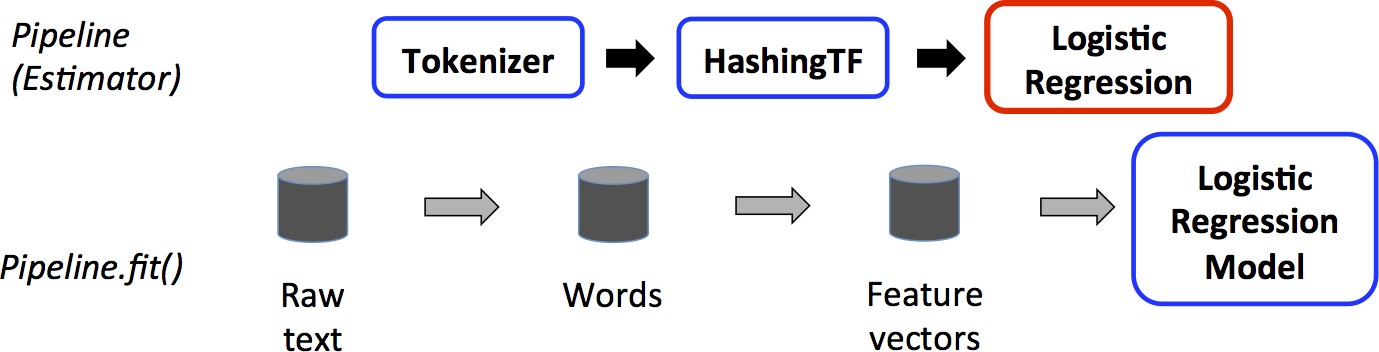
\includegraphics[width=\textwidth]{./bilder/ml-pipeline.png}}
  \caption{MLlib Pipeline \cite{SPMLLIB}}\label{fig:spark_ml_pipeline}
\end{figure}

\noindent
Ein Text wird eingelesen. In den ersten zwei Schritten (Tokenizer und HashingTF) arbeiten Transformatoren. Im dritten Schritt arbeitet ein Estimator (Logistic Regression). Die einzelnen Schritte werden im \autoref{sec_verbund} noch etwas genauer beschrieben.





\newpage
\subsection{Skalierung von R Programmen (SparkR)}\label{sec_sparkr}

\noindent
R hat den Nachteil, dass es zur Laufzeit nur auf einem einzelnen Thread arbeitet. Diese Hürde kann mit der SparkR Erweiterung genommen werden. SparkR ist ein R Paket, welches es ermöglicht, eine einfache Schnittstelle bereitzustellen, um Apache Spark von R auszunutzen. SparkR nutzt das bereits bekannte DataFrame, welches die Operationen wie \textsl{selection}, \textsl{filtering} oder \textsl{aggregation} bereitstellt. Das sind genau jene Operationen, die dem Anwender aus R bereits bekannt sind. \\
%Für große Datensätze kann SparkR zusätzlich auf maschinelles Lernen über MLlib zurückgreifen. \\

\noindent
Um das zu ermöglichen ist eine Brücke von R hin zum Spark Context bzw. den Nodes / Workern notwendig. Das Architekturschaubild in \autoref{fig:spark_r_architexture} zeigt diesen Ansatz. \\
\begin{figure}[h]
  \centering
  \fbox{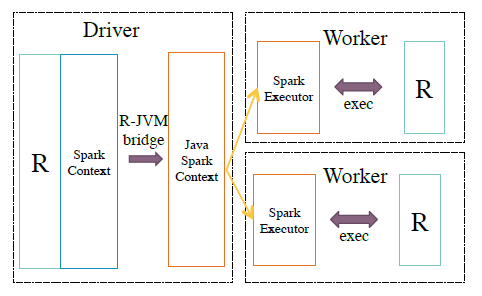
\includegraphics[width=100mm]{./bilder/spark_r_architecture.PNG}}
  \caption{SparkR Architektur \cite{VYL+16}}\label{fig:spark_r_architexture}
\end{figure}

\noindent
Die R-JVM bridge ermöglicht es von R aus Funktionen der JVM\footnote{\textbf{JVM} (java virtual machine) ist ein Teil der Java-Laufzeitumgebung. Der kompilierte Java-Bytecode wird innerhalb dieser virtuellen Maschinen ausgeführt.} aufzurufen. Somit wird vom R Spark Contex über die bridge zum Java Spark Context kommuniziert. Für die Kommunikation werden Sockets, die auf Netty\footnote{\textbf{Netty} ist ein High-Performance Netzwerk Framework} basieren, genutzt. Im Vergleich zu anderen Kommunikationsmethoden ist der zusätzliche Aufwand bei Sockets vergleichsweise gering und somit zu vernachlässigen.\footnote{Vgl. \cite{VYL+16}} \\
%Die Kommunikation üÜber die Sockets kann in beide Richtugnen kommuniziert werden und macht es m
%Es wurde in SparkR eine API geschaffen mit der es möglich . Das neue SparkR JVM System nutzt einen auf Netty basierenden Socket Server. Der Socket ansatz macht es möglich 

\noindent
Durch den Einsatz von SparkR kann die Verarbeitung auf vielen Rechnern verteilt stattfinden. Auch alle weiteren Merkmale wie In-Memory Cachings oder maschinelles Lernen können von Spark genutzt und ein großer Laufzeitgewinn erzielt werden. Bei einem Versuch wurden drei Abfragen mit acht bis 64 Kernen durchgeführt. Dabei konnte die Zeit von 115 Sekunden auf 20 Sekunden reduziert werden. Mit zusätzlichen Caching konnten die 20 Sekunden nochmal auf weniger als drei Sekunden reduziert werden\footnote{Vgl. \cite{VYL+16}}.

%Zusätzlich können alle bereits vorgestellten Komponenten auch über  kann bieten die Möglichkeiten, die 

%Solange Auswertungen in R nicht zeitkritisch sind ist der nutzen von SparkR nicht so hoch. Sobald aber Ausführungszeit ehr kurz sein muss oder einfach viel zu lang dauert 

\newpage
\section{Mehrere Komponenten im Verbund}\label{sec_verbund}

Nachdem die einzelnen Komponenten vorgestellt wurden, soll anhand eines praktischen Beispiels das Zusammenspiel verdeutlicht werden. \\
%Die Komponenten wurden jetzt einzeln vorgestellt. Jetzt soll das Zusammenspiel gezeigt werden. Hier bietet sich ein praktische Beispiel an. \\

\noindent
Es soll folgende Aufgabenstellung mit Apache Spark realisiert werden: Es gibt eine Datenmenge bestehend aus 100.000 Mitarbeiter-Datensätzen. Zu jedem Mitarbeiter sind Informationen wie Vorname, Nachname, Gehalt, Eintritt in die Firma, Adresse sowie Interessen/Hobbys bekannt. Diese Daten sind im strukturierten JSON\footnote{\textbf{JavaScript Object Notation (JSON)} ist ein kompaktes Datenformat für den Datenaustausch. }-Format hinterlegt. 
Aus diesem Datensatz sollen alle Mitarbeiter gefunden werden, die als Hobby Astrologie angegeben haben. Zusätzlich sollen diese auf keinen Fall Interesse an Autorennen und Bowling haben. Des Weiteren sollen die gefundenen Mitarbeiter nach ihrem Alter gruppiert werden. \\
Diese Aufgabenstellung macht es möglich die folgenden Komponenten zu nutzen:
\begin{itemize}
	\item die Kernklassen zum Sortieren und Reduzieren der Maps
	\item SparkSQL für das Einlesen der JSON-Datei und SQL-Abfragen
	\item SparkMLlib für das Trainieren der gesuchten Begriffe und finden der in Frage kommenden Mitarbeiter\footnote{Das Beispiel aus \cite{GITHUB_EXAMPLE} diente als Vorlage}	
\end{itemize}  

\noindent
Zuerst wird die SparkSession erzeugt und im Anschluss daran werden die Daten eingelesen. Neben JSON wären auch noch viele weitere Datenformate möglich gewesen (z.B.: csv, jdbc, text). Das lässt sich alles über die SparkCore realisieren. Der entsprechende Code-Block ist im Anhang in \autoref{code:verbund_1} zu sehen.\\

\noindent
Als nächstes wird eine Pipeline aufgebaut, in der ein PipelineModel so trainiert werden soll, dass es später aus dem Datensatz alle passenden Mitarbeiter mit möglichst hoher Trefferrate findet. Die Pipeline besteht aus drei Stages: Dem Tokenizer\footnote{Verarbeitet Text und teilt ihn in kleinere Stücke. In dem Fall in einzelne Worte, Auszug aus dem Datensatz: 'interests':'R/C Helicopters,Frisbee Golf – Frolf,Tetris'}, dem HashingTF\footnote{Erzeugt zu den Worten Hashes, um ein besseres Vergleichen zu ermöglichen.} und der LogisticRegression\footnote{Erzeugt eine Voraussage zu dem Datensatz gegenüber den Trainingsdaten.}. Nach dem Training werden die Daten in ein neues Dataset transformiert. In diesem Dataset sind die Vorhersagen enthalten. Die beschriebenen Schritte sind als Code im Anhang in \autoref{code:verbund_2} zu sehen. \\

\noindent
Zum Schluss werden die Mitarbeiter, die vorhergesagt wurden, per SparkSQL mit einer SQL Abfrage herausgefiltert und über MapReduce und Sortierung aus der SparCore Bibliothek in die endgültige Form gebracht. Das Implementierung dafür ist im \autoref{code:verbund_3} dargestellt. \\

\noindent
Es wurden 285 Mitarbeiter gefunden, die in Frage kommen. Darunter liegt der Großteil zwischen 25 und 35 Jahren. Das vollständige Ergebnis ist unter \autoref{code:verbund_3} zu finden.\\

\noindent
Die Komponenten greifen sehr gut ineinander. Die Schnittstellen und Funktionen wirken sehr einheitlich und es entsteht der Eindruck, dass das Hinzunehmen einer weiteren Spark Komponente kein Fremdkörper, sondern eine hilfreiche Ergänzung darstellt.

 
%In der Theorie sind die einzelnen Anwendunggebiet schön getrennt. Jedoch Die Anwendung der einzelnen Komponenten erscheint theoretisch 








